\section{JSON-Extract}
\label{sec:SchDisc}

This section describes JFUSE, our approach to discovering schema in JSON collections. Firstly, we show how to represent a schema collection as a data structure; we choose a graph structure representation. 

\subsection{Graph Representation}
\label{subsec:graph}

JSON collections may be easily viewed as a graph, where fields are vertices and sub-schema associated with a field are connected to the parent by edges. Furthermore, graphs allow a straightforward and fast way of traversing between parents, siblings, and children, which is highly valuable when building the proposed schema. 

The following definitions formalize how a JSON collection is loaded to the main memory.

\begin{definition} {\it JSON Graph}.
   A JSON graph is a directed graph built from a JSON collection defined by tuple \(G=(V, E)\). 
   \hfill{$\diamond$}
   \label{def:Graph}
\end{definition}

\begin{definition} {\it Vertex}. 
   A vertex \(\nu \in V\) is a tuple \(\nu\)\(=<l, \mathcal{T}, c, isEnum, isTU, \Lambda\)\(>\) where $l$ is the vertex's label and represents a field name, $\mathcal{T}$ is a tuple \(<\)\(t_1\):\(occ_1\), \(\ldots\), \(t_n\):\(occ_n\)$>$ (possibly unitary)  found in $l$ instances (where $t_i$:$occ_i$ is a key:value element that $t_i$ represents a type and $occ_i$ the number of occurrences of $t_i$ in $l$), $c$ is the number of occurrences of $l$ in the collection, \(isEnum\) indicates if \(l\) contents is an enumeration, \(isTU\) states if \(l\) defines a tagged union, and \(\Lambda\) stores a set (possibly empty) of possible values for l in V. 
   \hfill{$\diamond$}
   \label{def:GraphV}
\end{definition}

The following example illustrates how Definition~\ref{def:GraphV} is applied to build the vertices of our proposed graph.

\begin{example}
    Given the JSON collection from Figure~\ref{fig:JSONEx}, the following vertices belong to the graph built from the collection: \\
    %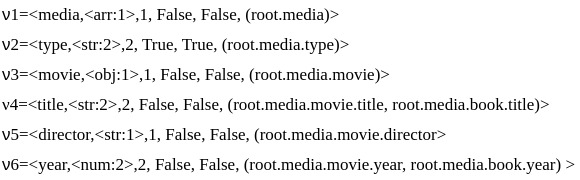
\includegraphics[scale=.43]{Figures/Vertices.jpg}
     \begin{itemize}
         \item \(\nu_1\)=$<$media,$<$arr:1$>$,1, False, False, NULL$>$
         \item \(\nu_2\)=$<$type,$<$str:2$>$,2, True, True, \{cinematography, text\}$>$
         \item \(\nu_3\)=$<$movie,$<$obj:1$>$,1, False, False, NULL$>$
         \item \(\nu_4\)=$<$title,$<$str:2$>$,2, False, False, NULL$>$
         \item \(\nu_5\)=$<$director,$<$str:1$>$,1, False, False, NULL$>$
         \item \(\nu_6\)=$<$year,$<$num:2$>$,2, False, False, NULL$>$
         \item \(\nu_7\)=$<$genres,$<$arr:2$>$,2, True, False, \{fantasy, adventure\}$>$        
     \end{itemize}
\end{example}
Note that the field \textit{type}, for example, appears twice in the collection, and in both cases, it is a string. The same goes for \textit{title} and \textit{year}. 

In the following, we define how a field becomes an enumeration and, if so, a tagged union. 
We use three thresholds to help discovering enumeration and tagged unions: (\textit{i}) \(thr_\Lambda\) to identify whether or not the content of a field may be an enumeration, (\textit{ii})  $Thr_t$ to indicate if the field content is dominated by a given type, and ($iii$) $Thr_{str}$  to check the length of the string in the content of a given field.

\begin{definition} {\it Enumeration}.
 A field from a JSON collection is set as an enumeration (i.e., \textit{isEnum} is true) if and only if  \(\nu \in V\) is associated with a set of values \(\Lambda\) such that: ($i$)  \(\mid\Lambda\mid\) \(\le thr_\Lambda\) and
 %($i$) given $c$ and \(|\Lambda|\), \(\frac{c}{|\Lambda|} \geq Thr_{rat}\),   
 ($ii$) let $t'$   in $\mathcal{T}$ be a tuple with a key:value $t_i$:$occ_i$:
 \begin{itemize}
     \item \(\frac{t'.occ_i}{\sum_{k=1}^{|\mathcal{T}|} t_k.occ_k}\) $\geq Thr_t$;
     \item If $t_i$ is a string type , let $\lambda'$ be the value with the maximum length in $\Lambda$,  $\lambda'$ $\leq$ $Thr_{str}$; and
     %\item If $t_i$ is a numeric type, it must be an integer with maximum of $\Lambda$,  $\lambda'$ $\leq$ $Thr_{int}$.
 \end{itemize}
   \hfill{$\diamond$}
   \label{def:Enum}
\end{definition}

The intuition behind Definition~\ref{def:Enum} is as follows: ($i$) the number of unique values of a given field cannot be greater than a threshold ($Thr_{\Lambda}$), ($ii$) the unique values must have a dominant type ($Thr_t$ $>=$ $n$\% where $n$ is the value), ($iii$) if the predominant type is a string, the length of the larger value cannot be greater than a threshold ($Thr_{str}$), since string enumerate values tend to be small, and ($iv$) float values tend not to compose enumeration values. 
For example, given the set of \textit{genres} values equals to \(\Lambda\)=\{\textit{fantasy, adventure}\},  $Thr_{\Lambda}$ equals 10, $Thr_{t}$ equals 0.8, and $Thr_{str}$ equals 20, \textit{genres} is considered an enumeration.

\begin{definition} {\it Tagged Union}.
A field from a JSON collection is set as a tagged union (i.e., isTU is true) if and only if $\nu \in V$ is an enumeration and its siblings respect the following: ($i$) let \(\lambda_1\) be a distinct value of vertex \(\nu\), so \(\nu.\lambda_1 \rightarrow v' \) are ensured in $G$. 
   \hfill{$\diamond$}
   \label{def:isTU}   
\end{definition}

The relationship \(\alpha \rightarrow \beta\) (\textit{i.e}, a functional dependency) from Definition~\ref{def:isTU} means that $\alpha$ determines the value of $\beta$. 
In our approach, we borrow the functional dependency definition from the database theory to state that, given two vertices \(\nu, \nu' \in V\) and $\lambda_1 \in \Lambda$ in $\nu$, \(\nu.\lambda_1\)  determines a sub-schema $\nu'$.

The following example shows the use of enumeration and tagged union.

\begin{example}
Given the JSON collection from Figure~\ref{fig:JSONEx}, the field \emph{type} is an enumeration since it comprises two distinct values: \emph{cinematography} and \emph{text}. And, it is a tagged union because when its value is cinematography, its right sibling is the field \emph{movie}; otherwise, it is the field \emph{book}. The relationships are \emph{type.cinematography}$\rightarrow$ \emph{movie} and \emph{type.text}$\rightarrow$ \emph{book}. 
On the other hand, the field \emph{genres} is also an enumeration; however, it is not a tagged union. 

\end{example}

\begin{definition} {\it Edge}. 
   An edge \(\varepsilon \in E\) is a tuple \(\varepsilon\)=\(<\)\((\nu_s\), \(\nu_t),\) \(rs, c_\varepsilon\), \(lv_\varepsilon\)\(>\) where (i) (\(\nu_s, \nu_t \in V\)) is a pair representing the source and target of the edge, respectively, (ii) \emph{rs} is the relationship between \(\nu_s\) and  \(\nu_t\) and can assume p or s indicating that \(\nu_s\) is parent or sibling of   \(\nu_t\), respectively, (iii) \(c_\varepsilon\) stores the number of occurrences of \emph{rs} between \(\nu_s\) and  \(\nu_t\), and (iv)  \(lv_\varepsilon\) is a list (possibly empty) that stores the values appearing when \(\nu_t\) is a sibling of \(\nu_s\).
   \hfill{$\diamond$}
   \label{GraphE}
\end{definition}

The components of a tuple in an edge $\varepsilon$ are used as follows: ($i$) \textit{rs} is employed in two flavors: first, to identify the sub-schema of a field when the relationship is $p$ or to determine if \(\nu_s\) is a tagged union candidate, ($ii$) \(c_\varepsilon\) controls whether or not a relationship $rs$ is mandatory (\(\frac{c_{\varepsilon}}{c~in~\nu_s} > Thr_m\)), \textit{i.e.}, the ratio of the number of occurrences of  $\nu_s$ and the number of occurrences of the relationship with  $\nu_t$ is greater than a threshold, and ($iii$) \(lv_\varepsilon\) is used to build a tagged union type.

\begin{example}
    Still using the JSON collection from Figure~\ref{fig:JSONEx}, the following edges belong to the built graph:
    \begin{itemize}
         \item \(\varepsilon_1\)=$<$(book, genres),p,2,NULL$>$
         \item \(\varepsilon_2\)=$<$(movie, director) ,p,1,NULL$>$
         \item \(\varepsilon_3\)=$<$(book, author),p,1,NULL$>$
         \item \(\varepsilon_4\)=$<$(type, book),s,1,(\textquotesingle text\textquotesingle)$>$
         \item \(\varepsilon_5\)=$<$(type, movie),s,1,(\textquotesingle cinematography\textquotesingle)$>$
    \end{itemize}
    
\end{example}

The above definitions state how we build a data structure to represent a JSON collection and use it to extract enumerations and tagged unions. 
Note that we need to set some thresholds (\textit{i.e.}, \(Thr_\Lambda\), \(Thr_t\), \(Thr_{str}\), and \(Thr_m\)) to allow our approach to work correctly. 
We run some experiments to identify the best values for the thresholds. 
In Section \ref{sec:ResDisc}, we present the values used in the main experiments.

Finally, Figure~\ref{fig:graphcoll} shows a graph representation from JSON collection in Figure~\ref{fig:JSONEx}. 
We use ellipses to represent all vertices, except for tagged unions represented by diamonds (field \textit{type}), enumeration by houses (field \textit{genres}), metadata as data by rectangles (vertices \textit{string} and \textit{numeric}), and vertices affected by tagged unions are reached by dotted edges (fields \textit{movie} and \textit{book}). 
Note that, for clarity, not all sibling edges appear in the graph, and we do not show the content of the vertices and edges.

\begin{figure*}[ht]
    \centering
    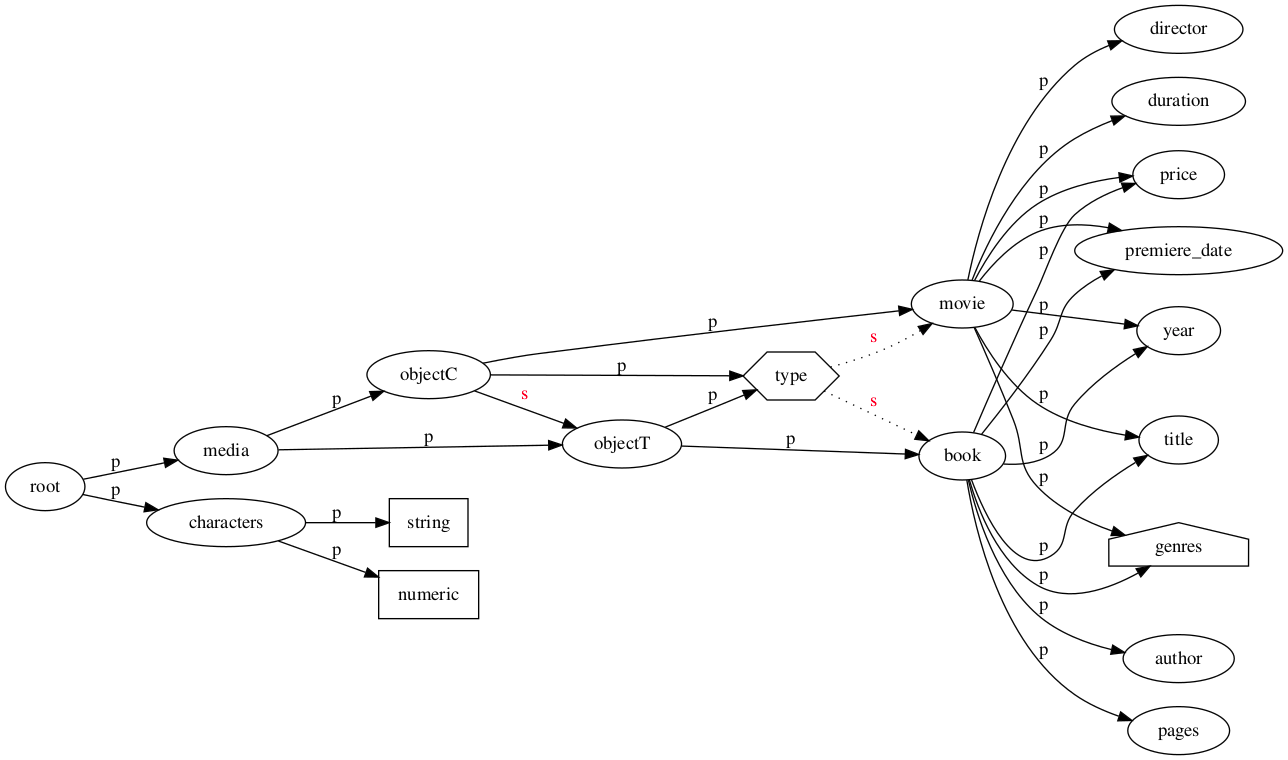
\includegraphics[scale=.35]{Figures/JSONgraph.png}
    \caption{Graph representing the collection in Figure~\ref{fig:JSONEx}.}
    \label{fig:graphcoll}
\end{figure*}

\subsection{Tuples, Collections, and Metadata}

Section~\ref{sec:prelim} shows that it is common sense that array types are composed of collections, and object types are composed of tuples. 
However, some JSON documents do not follow that. If the content of a given array $\mathcal{A}$ is very similar. The similarity is calculated based on the content type and a threshold (see Definition~\ref{def:Thrarr}).  
%(\textit{e.g.}, it contains only numeric atomic types), 
$\mathcal{A}$'s content can be seen as a tuple. 
The same reasoning can be applied to objects: if the content is dissimilar, it represents a collection of other objects. 
Besides, a sub-schema may represent data instead of metadata. 
For example, the content of field \textit{characters} is not a list of \textit{field:value}; it is a list of names with ages, and, in this case, they are not metadata. 
We cannot extract a rule like \textit{characters}: \{``harry potter'': integer ``hermione granger'': integer\} because the characters' names and ages represent data. 
In the following, we formalize some definitions to identify when content is a tuple or a collection. When it is a tuple, the content may be considered data.

\begin{definition}
 \label{def:Thrarr}
    Array as Tuple. Given an array content $\mathcal{C}$, $\mathcal{C}$ is seen as a tuple if and only if ~$\mathcal{C}$ is composed of ~$Thr_{arr}$ of same elements.   \hfill{$\diamond$}
\end{definition}

Note that, from the definition, when the content of an array is very similar, we can consider it as a tuple. 
A threshold is used to take into account noise in the content. 
%Based on our experiments, 90\% (\textit{i.e.}, 0.9) is a reasonable threshold.

\begin{definition}
    Object as Collection. Given an object content $\mathcal{C}$, $\mathcal{C}$ is seen as a collection if and only if ~$\mathcal{C}$ contains ~$Thr_{obj}$ of dissimilar elements.   \hfill{$\diamond$}
\end{definition}

Note that from the definition, when the content of an object contains some dissimilarity, we can consider it as a collection.  
The threshold $Thr_{obj}$ is used to take into account noise in the content. 
%Based on our experiments, over 10\% (\textit{i.e.}, 0.1) is a reasonable threshold.

Finally, we define the problem of data being represented as metadata. This problem was raised in~\citep{Nam21,Sp+21}, and the goal is to find when a JSON sub-schema represents data instead of metadata.

\begin{definition}
    Metadata as data. Given a content \(\mathcal{C}\) of an object seen as a collection, if \(\mathcal{C}\) is composed only of $<$key$>$:$<$value$>$ and more than $Thr_{dt}$\% are optional,  \(\mathcal{C}\) represents data instead of metadata in the collection. 
    \label{def:metadata}
    \hfill{$\diamond$}
\end{definition}

Note that, from Definition~\ref{def:metadata}, the threshold  \(Thr_{dt}\)\% plays an essential role in considering a pair $<$\textit{key}$>$:$<$\textit{value}$>$ as data instead of metadata.  
For example, if a label \textit{L} occurs 50 times, its child \textit{Lc} occurs 48 times, and $Thr_{dt}$\% is set to 95, \textit{Lc} would be mandatory.
 
The content of the field \textit{characters} (Line 23 in Figure~\ref{fig:JSONEx}) is a case of metadata as data: the characters name and age are data. Representing them as metadata, we should use another type of representation, for example, $<$name$>$:\(\mathbb{R}\). 
Instead, the model is \(\mathbb{S}\):\(\mathbb{R}\). 
The optionality of the content leads our approach to consider it as data or metadata. 
%The threshold $Thr_{dt}$ is used for that. %to 70\% to identify whether or not a sub-schema represents data.  

\subsection{JSON Metamodel}
\label{subsec:meta}

We propose a metamodel to represent a conceptual schema for JSON collections. 
Our metamodel is expressed using BNF-like metasyntax (Backus-Naur form). 
BNF is a formal way to describe a language and, in our approach, a JSON schema. 
It consists of a set of terminal and non-terminal symbols. 
The symbols derive a language using production rules in the form \textit{left-hand-side::=right-hand-side}, where LHS (Left-Hand-Side) is a non-terminal symbol, and RHS (Right-Hand-Side) is a sequence of symbols (terminals or non-terminals). 
The meaning of a production rule is the LHS (a non-terminal symbol) may be replaced by the expression represented by RHS.

Accordingly, our meta JSON schema language is defined as follows:
%\setlength{\grammarparsep}{20pt plus 1pt minus 1pt} % increase separation between rules
\setlength{\grammarindent}{81pt} % increase separation between LHS/RHS 
\begin{grammar}
\parsep\grammarparsep
<atm-type> ::= $\mathbb{S}$ | $\mathbb{R}$ | $\mathbb{B}$ | \textit{null}

<field-name> ::= $(\mathbb{S})^+$

<atm-field> ::= <field-name> `:' <at-type>

<arr-type> ::= `[' <arr-value>, $\dots$, <arr-value> `]'

<arr-value> ::= (<atm-type> | <arr-type> | <obj-type>)$^+$

<array> ::= <field-name> `:' <arr-type>

<obj-type> ::= `{' (<atm-field> | <array> | <object>)$^+$ `}'

<object> ::= <field-name> `:' <obj-type>
\end{grammar}

\noindent where ($i$) \(<\)\textit{atm-type}\(>\)  defines the atomic types $\mathbb{S}$, $\mathbb{R}$, $\mathbb{B}$, and  \textit{null} represent a string, numeric, boolean, and null value, respectively and  ($ii$) \(<\)\textit{field-name}\(>\) represents a valid field name in JSON collections. The other constructors follow the same reasoning. 


Finally, enumeration and tagged union production rules can be defined as follows:

\setlength{\grammarindent}{95pt} % increase separation between LHS/RHS 
\begin{grammar}
\parsep\grammarparsep
<enum> ::= <field-name> `:[' <atm-type>, $\dots$, <atm-type> `]'

<tagged-union> ::= `IF' <enum-cond> `THEN' (<atm-field> | <array> | <object>)

<enum-cond> ::= <field-name> `.' <atm-type>
\end{grammar}

The following example shows an instance of our metamodel representing the JSON collection from our running example (Figure~\ref{fig:JSONEx}).

\begin{example}
    ~ \\ \\
    root \hspace{20pt} \textnormal{::=} \{\textbf{media:} arr\_m \textbf{characters:} str\_ch\}\\
    arr\_m \hspace{8pt}  \textnormal{::=}  \textnormal{[}obj\_a\textnormal{]} \\
    obj\_a \hspace{10pt} \textnormal{::=} IF \textbf{type.cinematography} THEN obj\_c \\
    \hspace*{52pt} $\mid$ IF \textbf{type.text} THEN obj\_t \\
    obj\_c \hspace{12pt} \textnormal{::=} \textbf{movie:} obj\_m \\
    obj\_t \hspace{14pt} \textnormal{::=} \textbf{book:} obj\_b \\
    obj\_m \hspace{9pt}  \textnormal{::=} \textbf{title:}$\mathbb{S}$ ~\textbf{director:}$\mathbb{S}$ ~\textbf{year:}$\mathbb{R}$ ~\textbf{premiere\_date}:arr\_date~\textbf{duration:}$\mathbb{R}$ \\
    \hspace*{60pt} \textbf{price:} $\mathbb{N}$ \textbf{genres}:arr\_g \\
    %enum\_g:=\textbf{fantasy} $\mid$ \textbf{adventure} \\
    obj\_b \hspace{11pt} \textnormal{::=} \textbf{title:}$\mathbb{S}$ ~\textbf{author:}$\mathbb{S}$ ~\textbf{year:}$\mathbb{R}$ ~\textbf{premiere\_date}:arr\_date~\textbf{pages:}$\mathbb{R}$ ~\textbf{price:}$\mathbb{R}$ \\
    \hspace*{60pt} \textbf{genres}:~arr\_g\\
    arr\_g \hspace{11pt} \textnormal{::=} \textnormal{[}\textbf{fantasy} , \textbf{adventure}\textnormal{]} \\
    arr\_date \textnormal{::=} \textnormal{[}$\mathbb{R}$, $\mathbb{R}$, $\mathbb{R}$\textnormal{]} \\
    str\_ch \hspace{9pt} \textnormal{::=} \{\textnormal{(}$\mathbb{S}$ \textnormal{:} $\mathbb{R}$\textnormal{)}$^+$\}%\\
\end{example}

Note that \textit{obj\_a} represents a tagged union, \textit{arr\_g} represents an enumeration, \textit{str\_ch} is modeled as pairs \textit{string:string} because the field \textit{characters} is considered a collection and not an object, and \textit{arr\_date} models a tuple encoded in an array representing a date type (MM, DD, YYYY). 
A na\"ive approach would extract \textit{arr\_date} as [$\mathbb{R}(,\mathbb{R})^*$], that is, a sequence of numerical values.